\chapter{Demodulation Algorithms}
After discussing the different demodulation techniques it is time to have some more discussion of software based demodulation techniques, specifically. However, before talking about the algorithms for doing the FSK demodulation it is worth specifying what type of FSK Bell 202 is. There are two features that are relevant for taking into consideration when demodulating the signal. First, is that it is asynchronous meaning that there is no separate clocking signal and it is embedded within the data signal. If it were synchronous there would be two different signals coming into the demodulator which would be the data carrier signal and a clocking signal. The second characteristic is that the FSK is coherent or continuous. This means that there is a continuous signal at bit boundaries and there are no jumps as the signal changes from one frequency to another as seen in Figure \ref{coherentFSKExample} as opposed to non-coherent Figure \ref{noncoherentFSKExample}. Another name sometime applied to this method of FSK is continuous-phase frequency shift keying or CPFSK \cite{WikipediaCPFSK}. It might be noticed that some of the figures used in the discussion previously also exhibited the coherent characteristic. The next few sections are general approaches that can be used for any FSK demodulation. In addition to describing each generally some specific details of APRS Bell 202 demodulation. 
\begin{figure}
  \centering
	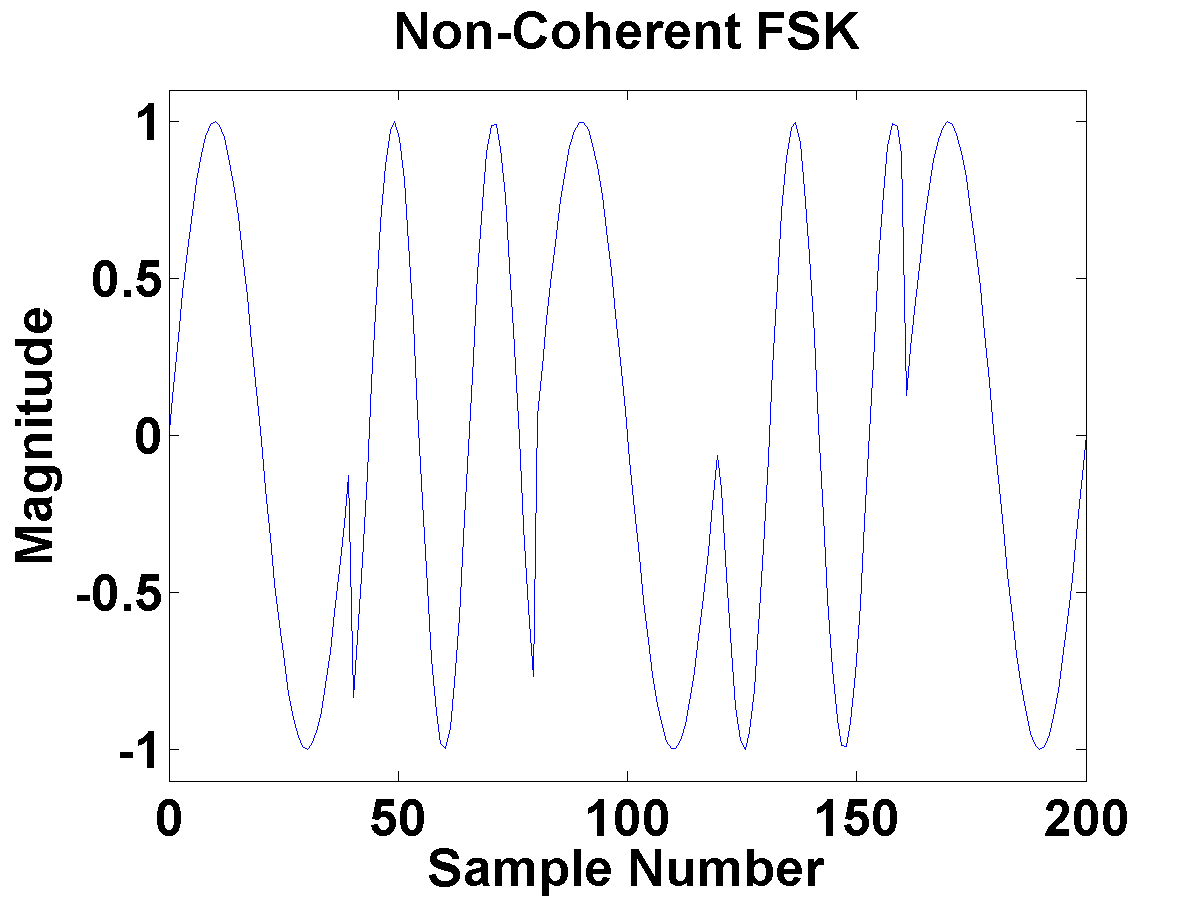
\includegraphics[width=0.75\linewidth]{images/NonCoherentFSK.png} 
	\caption{Example of a non-coherent 1200Hz / 2200Hz FSK signal.}
   \label{noncoherentFSKExample}
\end{figure}
\begin{figure}
  \centering
	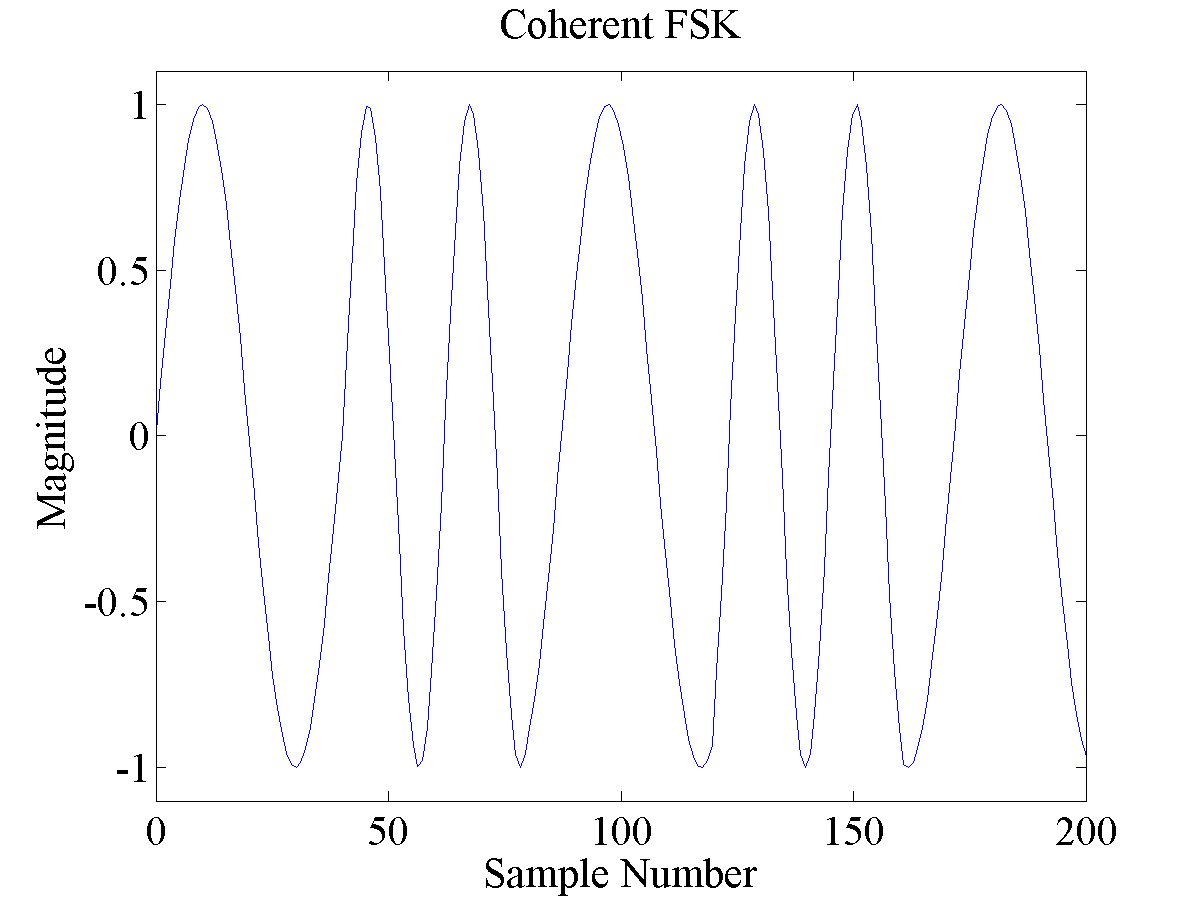
\includegraphics[width=0.75\linewidth]{images/CoherentFSK.png} 
	\caption{Example of a non-coherent 1200Hz / 2200Hz FSK signal.}
   \label{coherentFSKExample}
\end{figure}

\section{Zero Crossing}
Using zero crossings to determine the frequency of the FSK signal is one of the the easiest algorithms from a software implementation perspective. The idea is that based off of the time elapsed between zero crossings of the signal the period of the waveform can be measured. Once the period has been calculated the frequency can then be easily calculated using the inverse relationship between period and frequency, \textit{f} = 1 /T where \textit{f} is the frequency and T is the period. It is worth noting and keeping in mind that two consecutive zero crossings are only half of the period since there are a total of three zero crossings in one period.

\section{Correlation}
Another method that can be used for demodulation of FSK is correlation with the underlying FSK signals. For APRS this is done by synthesizing a 1200Hz tone and a 2200Hz tone and then comparing the input signal to each of these. Which ever one of the synthesized signals the input signal is more similar to - has more correlation with - the input signal must be the frequency that is present at that point in time in the data carrying signal. 

\section{Discrete Fourier Transform}
A discrete Fourier Transform is one implementation of Fourier Transform that is executed on discrete samples similar to what is present in a digital audio file. Once a Fourier transform has been applied on a signal the output is a relative power versus frequency. With this data which ever frequency, either 1200Hz or 2200Hz, is more prominent is which symbol must be present in the bit period.

\subsection{Goertzel Algorithm}
Computing a discrete Fourier transform is more reasonable computationally than a full Fourier transform which is an integral as opposed to having discrete terms \cite{WikipediaFT}. However, even the results from the DFT could have more data than is needed to do the demodulation since the results will be a spectrum of powers over a range of frequencies \cite{WikipediaDFT,WikipediaFFT}. A more simplified and specified approach can be used. The Goertzel Algorithm evaluates the coefficients and corresponding powers of the individual frequencies of 1200Hz and 2200Hz \cite{WikipediaGA,Elmenreich2011}. 

\section{Phase Lock Loop}
A phase lock loop (PLL) is exactly what the name implied. It is a loop that stays locked onto the phase of the input signal. This is done by taking input signal detecting the phase and then producing an output the corresponds with the phase. The output is fed back in with the input so that any differences between the input and output of the phase lock loop can be reconciled to have a phase exactly in phase with the input. The convenient thing about monitoring the phase of the signal so closely and being able to stay locked onto it is that the frequency must also be known. Extracting this frequency information from the PLL can hence be used for FSK demodulation.

\section{Advantages of Using the Derivative of the Original Signal}
One thing considered while trying to demodulate the Bell 202 signals was the implications of using the derivative of the signal for decoding as opposed to the actual signal. One advantage that was seen through using this approach is that for cases where there is a DC offset of the signal, the derivative would remove this and re-center the signal about zero. A consequence of using the derivative of a sine wave signal is that the result will be 90 degrees out of phase. It was decided that this would not be a problem since the whole signal would be 90 shifted by this amount and the timing is done on the fly once the signal is received anyways. However, there were some other things about using the derivative that were not considered until later. One thing is that in addition to to helping the DC offset it also helps signals that were de-emphasized by not pre-emphasized. In signals where this is the case the 2200Hz tones will be lower in the original signal, but since they have a steeper slope this ends up helping to normalize these differences in the resulting derivative. An example showing this problem as well as a DC offset in the data signal and its derivative can be seen in Figure \ref{emphasisAndDerivativeExample}. Although the derivative helps with this, it will hurt if the opposite is the case (preemphasized but not deemphasized) only worsening the problem.
\begin{figure}
  \centering
	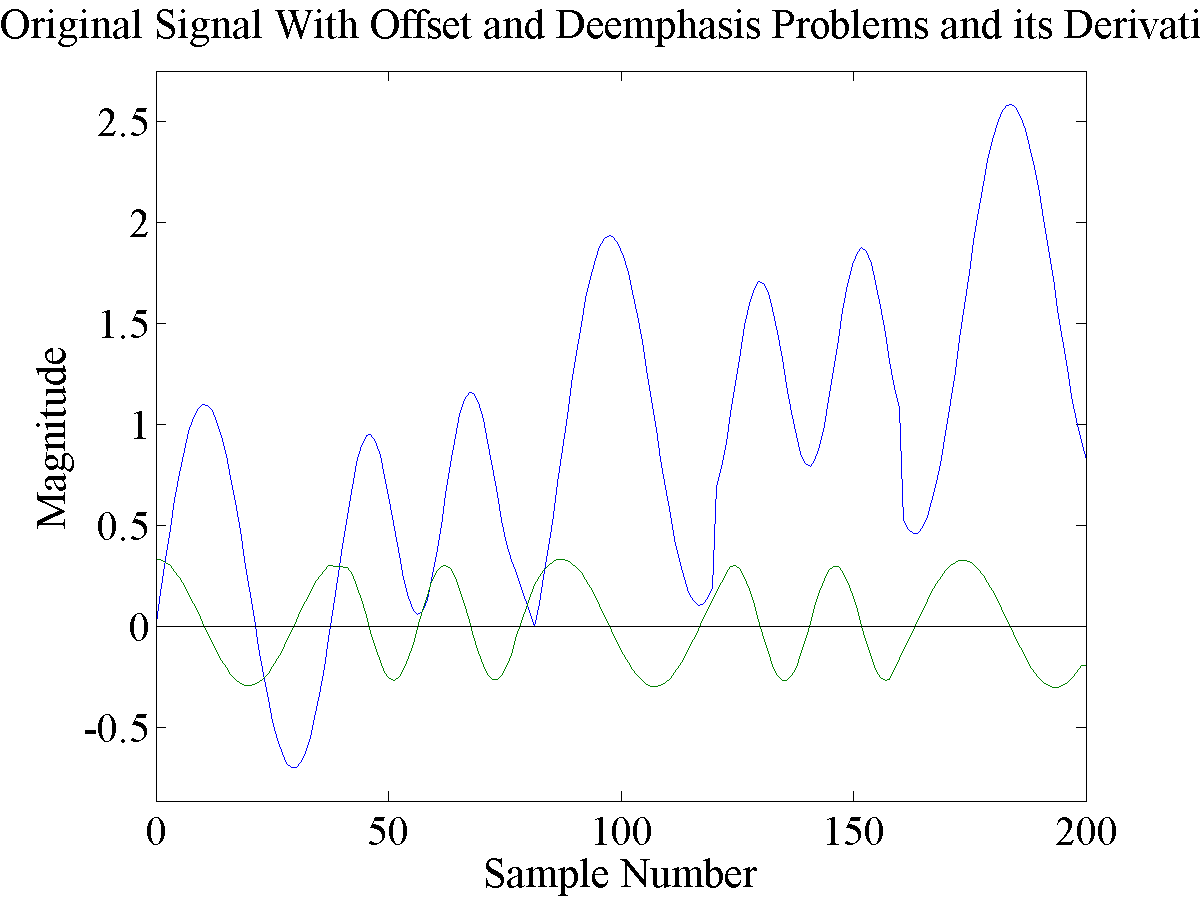
\includegraphics[width=0.75\linewidth]{images/OriginalSignalWithOffsetandDeemphasisProblemsanditsDerivative.png} 
	\caption{Example of a signal that has both a DC offset and a deemphasis problem and its corresponding derivative.}
   \label{emphasisAndDerivativeExample}
\end{figure}

\section{Additional Benefits of Software Based Decoding}
Software is flexible. Any one of the aforementioned algorithms can be used on the same hardware without having to add additional discrete components, add new Integrated Circuits (ICs), or make modifications to a Printed Circuit Board (PCB). There are a two benefits of using software instead of dedicated hardware that this research will investigate; first exhaustive search of a signal through the use of buffers, and second, the ability to be able to run multiple of these demodulation approaches in parallel.

\subsecion{Exhaustive Search of Incoming Signal}
Using software the input signal can be buffered in the program and then searched for a signal. Since there is not a separate data and clock signal, there could be a case when the clocking is improperly selected. Using an approach of buffering data that may contain a valid packet, the software can step through the data trying every possible clocking option.

\subsection{Taking Advantage of Parallel Demodulation}
Another potential advantage of using software for decoding these AFSK signal is being able to apply multiple demodulation techniques. Once the data is collected in coverted to a digital form there is no reason, other than computation limitations of the host computer, not to run multiple algorithms in parallel in order to be able to demodulate the maximum number of packets possible. Although there are packets that every algorithm is able to decode, there are also those that some approaches can decode while others can not. Through using multiple in parallel for demodulation and de-duplicating the demodulated results even more packets can be correctly decoded.
